\documentclass[11pt,a4paper]{article}

\usepackage[utf8]{inputenc}
\usepackage[T1]{fontenc}
\usepackage[ngerman]{babel}
\usepackage{lmodern}
\usepackage{amsmath,amssymb}
\usepackage{graphicx}
\usepackage{booktabs,tabularx,array}
\usepackage[table]{xcolor}
\usepackage{tikz}
\usetikzlibrary{arrows.meta,positioning,shapes.geometric,calc}
\usepackage[most]{tcolorbox}
\usepackage{enumitem}
\usepackage{microtype}
\usepackage{hyperref}
\usepackage[a4paper,left=18mm,right=18mm,top=15mm,bottom=15mm,headheight=0pt]{geometry}

\definecolor{navy}{HTML}{174A63}
\definecolor{blue}{HTML}{2E7698}
\definecolor{lightblue}{HTML}{EAF3F7}
\definecolor{lightgray}{HTML}{F2F3F4}
\definecolor{midgray}{HTML}{66727A}
\definecolor{green}{HTML}{477A63}
\definecolor{orange}{HTML}{B96A2B}

\hypersetup{colorlinks=true,linkcolor=navy,urlcolor=blue,pdftitle={Sicherungsblatt Aufgabe 2 -- Trainings- und Testdaten}}
\setlength{\parindent}{0pt}
\setlength{\parskip}{4pt}
\setlist[itemize]{leftmargin=5mm,itemsep=1.5pt,topsep=2pt}
\setlist[enumerate]{leftmargin=6mm,itemsep=2pt,topsep=2pt}
\renewcommand{\familydefault}{\sfdefault}

\pagestyle{empty}

\newtcolorbox{definition}[1][]{enhanced,breakable,colback=lightblue,colframe=blue,
  boxrule=0.8pt,arc=1.5mm,left=3mm,right=3mm,top=2mm,bottom=2mm,
  fonttitle=\bfseries,title=Definition,#1}
\newtcolorbox{merke}[1][]{enhanced,breakable,colback=lightgray,colframe=navy,
  boxrule=0.9pt,arc=1.5mm,left=3mm,right=3mm,top=2mm,bottom=2mm,
  fonttitle=\bfseries,title=Merke,#1}
\newtcolorbox{beispiel}[1][]{enhanced,breakable,colback=white,colframe=midgray,
  boxrule=0.7pt,arc=1.5mm,left=3mm,right=3mm,top=2mm,bottom=2mm,
  fonttitle=\bfseries,title=Beispiel,#1}
\newtcolorbox{ueberblick}[1][]{enhanced,breakable,colback=lightblue,colframe=navy,
  boxrule=1.1pt,arc=1.5mm,left=3mm,right=3mm,top=2.5mm,bottom=2.5mm,
  fonttitle=\bfseries,title=Überblick,#1}

\newcommand{\fach}[1]{\textbf{\color{navy}#1}}
\newcommand{\sectionline}[1]{%
  \vspace{1mm}{\Large\bfseries\color{navy}#1}\par\vspace{1mm}%
  {\color{blue}\rule{\linewidth}{0.8pt}}\vspace{1mm}}
\newcommand{\sheettitle}[2]{%
  \begin{tcolorbox}[colback=navy,colframe=navy,arc=2mm,boxrule=0pt,left=5mm,right=5mm,top=2.5mm,bottom=2.5mm]
    {\color{white}\fontsize{20}{24}\selectfont\bfseries #1}\par
    \vspace{0.5mm}{\color{white}\large #2}
  \end{tcolorbox}}
\newcommand{\subline}[1]{\vspace{1mm}{\large\bfseries\color{navy}#1}\par}

\begin{document}

\sheettitle{Zwei Bäume im Vergleich}{Entscheidungsbäume · Sicherungsblatt zu Aufgabe 2 · Informatik 11}

\sectionline{1. Trainings- und Testdaten}

Die verfügbaren gelabelten Daten werden getrennt verwendet:

\begin{itemize}
  \item \fach{Trainingsdaten} sind gelabelt bzw. beschriftet und werden zur Erzeugung des Modells verwendet.
  \item \fach{Testdaten} sind gelabelt bzw. beschriftet und werden zur Beurteilung der Vorhersagequalität verwendet.
\end{itemize}

\begin{beispiel}[title=Beispiel: gelabelte Trainingsdaten]
Die bekannten Äffchen sind mit den Labels \emph{beißt} oder \emph{beißt nicht} versehen. Aus diesen
Beispielen kann ein Entscheidungsbaum Regeln für die Klassifikation neuer Äffchen lernen.

\begin{center}
  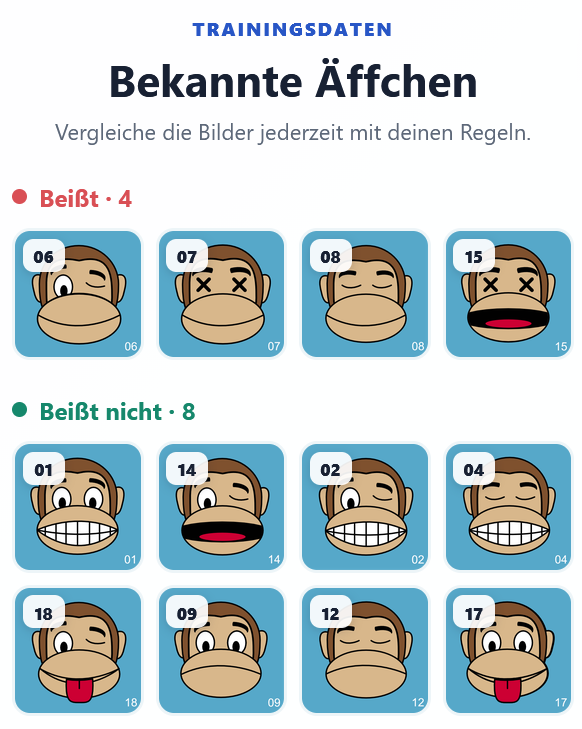
\includegraphics[width=0.52\linewidth]{sicherungsblatt-bilder/trainingsdaten-bekannte-aeffchen.png}

  {\scriptsize\color{midgray}Beispielgrafik: Äffchen-Illustrationen im Ausgangsmaterial von Annabel Lindner und Stefan Seegerer, CC BY-NC.}
\end{center}
\end{beispiel}

\begin{merke}
Die Trennung verhindert, dass ein Modell nur an bereits bekannten Daten gut wirkt. Erst neue Testdaten zeigen,
wie zuverlässig seine \fach{Vorhersagen} sind. \\
Zwei Entscheidungsbäume können dieselben Trainingsdaten vollständig richtig klassifizieren und bei unbekannten
Testdaten trotzdem unterschiedlich gut funktionieren. \\ Die Trainingsdaten müssen nicht jede mögliche
Merkmalskombination enthalten.
\end{merke}

\end{document}
